In contrast to conventional, coin-based quantum walks, which proceed straightforwardly from one vertex to another, the staggered variant  \cite{PortugalSFG16} takes advantage of forming partitions of graph cliques\footnote{A clique is a subset of vertices of an
undirected graph such that every two distinct vertices are adjacent.} over the graph structure of the walking space. Each partition forms a tesselation whose elements do not overlap. The set of
cliques in each tessellation must cover all vertices of the graph, and the set
of tessellations $\{T_{1}$,$T_{2}$, \ldots ,$T_{k}\}$ chosen
must cover all the edges.

Then  a unit vector, typically encoding a uniform
superposition, is associated to each clique so that
the vector belongs to the subspace spanned by the corresponding vertices; i. e., 
\begin{equation}
	\ket{u_{j}^{k}} = \frac{1}{\sqrt{\mathopen|\alpha_{j}^{k}}\mathclose|}\sum_{l\in\alpha_{j}^{k}}\ket{l},
\end{equation}
where $\alpha_{j}^{k}$ is the $j^{th}$ polygon in the $k^{th}$ tessellation.

This way each tessellation $k$ gives rise to an operator 
\begin{equation}
	H_k = 2\sum_{j=1}^{p}\ket{u_{j}^{k}}\bra{u_{j}^{k}} - I.
	\label{eq:StagHamil}
\end{equation}
which propagates the probability amplitude locally, in each clique.
The composition of all such operators defines the evolution operator, which, by solving the 
the time-independent Schr\"odinger equation, is equivalent to 
\begin{equation}
	U = e^{i\theta_{k}H_{k}}...e^{i\theta_{2}H_{2}}e^{i\theta_{1}H_{1}}, \text{  where  }\; e^{i\theta_{k}H_{k}} = \cos{(\theta_k)}I + i\sin{(\theta_k)}H_k
	\label{eq:stagWalkUnmodOp}
\end{equation}
since $H_k^2 = I$, meaning that the Hamiltonian is a reflection operator that,
when expanded in a Taylor series, generates a local operator.

As an elementary example consider a line where the following two tessellations  (depicted in red and blue below) are defined 
\begin{equation}
	T_{\alpha}= \{\{2x,2x+1\}\colon x \in \mathbb{Z}\}\; \; \text{and}\; \; T_{\beta}= \{\{2x+1,2x+2\}\colon x \in \mathbb{Z}\}.
\end{equation}

\begin{center}
	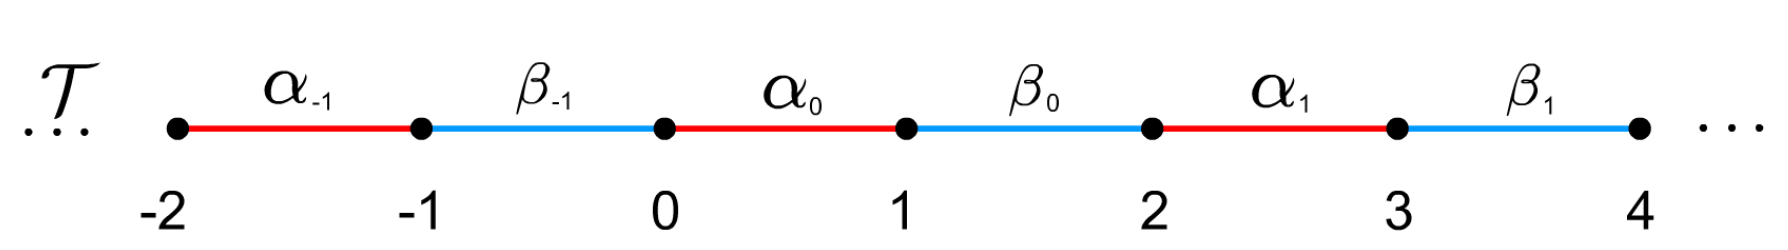
\includegraphics[scale=0.30]{img/tesselation.png}
\end{center}
Thus, 
\begin{equation}
	\ket{\alpha_x} = \frac{\ket{2x} + \ket{2x+1}}{\sqrt{2}}\; \; \text{and}\; \; \ket{\beta_x} = \frac{\ket{2x+1}+\ket{2x+2}}{\sqrt{2}},
\end{equation}
yielding Hamiltonians 
\begin{equation}
	H_\alpha = 2\sum_{x=-\infty}^{+\infty}\ket{\alpha_{x}}\bra{\alpha_x} - I \; \; \text{and}\; \;  H_\beta = 2\sum_{x=-\infty}^{+\infty}\ket{\beta_{x}}\bra{\beta_x} - I.
\end{equation}

Therefore, $U = e^{i\theta H_\beta}e^{i\theta H_\alpha}$ is the  evolution operator. The probability
distribution  on a line after 50 steps, starting at $\ket{+}$, for different values of $\theta$, is depicted below,    
noticing that the walker is more likely to be found further away from the origin
as the angle increases.
\begin{center}
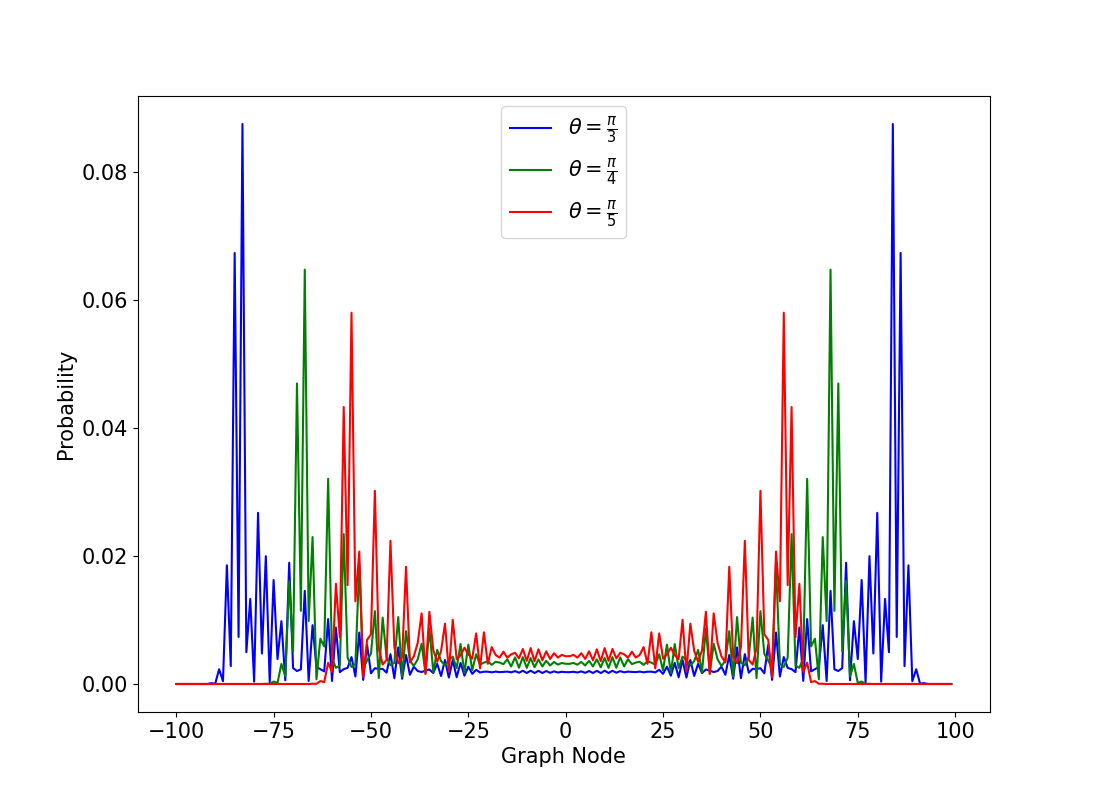
\includegraphics[scale=0.30]{img/stagqwMultiple.png}
\end{center},


